%% BioMed_Central_Tex_Template_v1.06
%%                                      %
%  bmc_article.tex            ver: 1.06 %
%                                       %

%%IMPORTANT: do not delete the first line of this template
%%It must be present to enable the BMC Submission system to
%%recognise this template!!

%%%%%%%%%%%%%%%%%%%%%%%%%%%%%%%%%%%%%%%%%
%%                                     %%
%%  LaTeX template for BioMed Central  %%
%%     journal article submissions     %%
%%                                     %%
%%          <8 June 2012>              %%
%%                                     %%
%%                                     %%
%%%%%%%%%%%%%%%%%%%%%%%%%%%%%%%%%%%%%%%%%


%%%%%%%%%%%%%%%%%%%%%%%%%%%%%%%%%%%%%%%%%%%%%%%%%%%%%%%%%%%%%%%%%%%%%
%%                                                                 %%
%% For instructions on how to fill out this Tex template           %%
%% document please refer to Readme.html and the instructions for   %%
%% authors page on the biomed central website                      %%
%% http://www.biomedcentral.com/info/authors/                      %%
%%                                                                 %%
%% Please do not use \input{...} to include other tex files.       %%
%% Submit your LaTeX manuscript as one .tex document.              %%
%%                                                                 %%
%% All additional figures and files should be attached             %%
%% separately and not embedded in the \TeX\ document itself.       %%
%%                                                                 %%
%% BioMed Central currently use the MikTex distribution of         %%
%% TeX for Windows) of TeX and LaTeX.  This is available from      %%
%% http://www.miktex.org                                           %%
%%                                                                 %%
%%%%%%%%%%%%%%%%%%%%%%%%%%%%%%%%%%%%%%%%%%%%%%%%%%%%%%%%%%%%%%%%%%%%%

%%% additional documentclass options:
%  [doublespacing]
%  [linenumbers]   - put the line numbers on margins

%%% loading packages, author definitions

%\documentclass[twocolumn]{bmcart}% uncomment this for twocolumn layout and comment line below
\documentclass{bmcart}

%%% Load packages
%\usepackage{amsthm,amsmath}
%\RequirePackage{natbib}
%\RequirePackage[authoryear]{natbib}% uncomment this for author-year bibliography
%\RequirePackage{hyperref}
\usepackage[utf8]{inputenc} %unicode support
%\usepackage[applemac]{inputenc} %applemac support if unicode package fails
%\usepackage[latin1]{inputenc} %UNIX support if unicode package fails
%\usepackage{lineno}
%\linenumbers
%\linespread{2}


\usepackage[percent]{overpic}
\usepackage{graphicx}
\usepackage{color}
\usepackage{todonotes}
\usepackage{verbatim}
\usepackage[english]{babel}
\usepackage{caption}
\usepackage{float}
\usepackage{url}
\usepackage{tcolorbox}
\usepackage{hyperref}
\usepackage[]{algorithm2e}
\usepackage{amsmath}
\usepackage{amsfonts} %%% added by Fanny to get mathsbb 

%%%% remove this line when submitting
\newcommand{\fanny}[1]{\textcolor{blue}{*** FP: #1}}

%%%%%%%%%%%%%%%%%%%%%%%%%%%%%%%%%%%%%%%%%%%%%%%%%
%%                                             %%
%%  If you wish to display your graphics for   %%
%%  your own use using includegraphic or       %%
%%  includegraphics, then comment out the      %%
%%  following two lines of code.               %%
%%  NB: These line *must* be included when     %%
%%  submitting to BMC.                         %%
%%  All figure files must be submitted as      %%
%%  separate graphics through the BMC          %%
%%  submission process, not included in the    %%
%%  submitted article.                         %%
%%                                             %%
%%%%%%%%%%%%%%%%%%%%%%%%%%%%%%%%%%%%%%%%%%%%%%%%%


%\def\includegraphic{}
%\def\includegraphics{}



%%% Put your definitions there:
\startlocaldefs
\newcommand{\review}[1]{\textcolor{black}{#1}}
\newcommand{\revieww}[1]{\textcolor{red}{#1}}
\newcommand{\mb}[1]{\boldsymbol{\mathbf{#1}}}
\DeclareUnicodeCharacter{00A0}{~}
\endlocaldefs


%%% Begin ...
\begin{document}

%%% Start of article front matter
\begin{frontmatter}

\begin{fmbox}
\dochead{Method}

%%%%%%%%%%%%%%%%%%%%%%%%%%%%%%%%%%%%%%%%%%%%%%
%%                                          %%
%% Enter the title of your article here     %%
%%                                          %%
%%%%%%%%%%%%%%%%%%%%%%%%%%%%%%%%%%%%%%%%%%%%%%

\title{Unlocking RNA-seq tools for zero-inflation and single cell applications using observation weights}

%%%%%%%%%%%%%%%%%%%%%%%%%%%%%%%%%%%%%%%%%%%%%%
%%                                          %%
%% Enter the authors here                   %%
%%                                          %%
%% Specify information, if available,       %%
%% in the form:                             %%
%%   <key>={<id1>,<id2>}                    %%
%%   <key>=                                 %%
%% Comment or delete the keys which are     %%
%% not used. Repeat \author command as much %%
%% as required.                             %%
%%                                          %%
%%%%%%%%%%%%%%%%%%%%%%%%%%%%%%%%%%%%%%%%%%%%%%

\author[
   addressref={aff1,aff2},                   % id's of addresses, e.g. {aff1,aff2}
   %corref={aff1,aff2},                       % id of corresponding address, if any
   noteref={n1},                        % id's of article notes, if any
   email={koen.vandenberge@ugent.be}   % email address
]{\inits{KVdB}\fnm{Koen} \snm{Van den Berge}}
\author[
    addressref={aff3},
       noteref={n1},
    email={fperraudeau@berkeley.edu}
]{\inits{FP} \fnm{Fanny} \snm{Perraudeau}}

\author[
    addressref={aff4,aff5},
    email={charlotte.soneson@uzh.ch}
]{\inits{CS} \fnm{[TBD POSITIONS] Charlotte} \snm{Soneson}}
\author[
    addressref={aff6},
    email={milove@email.unc.edu}
]{\inits{ML} \fnm{Michael I.} \snm{Love}}
\author[
    addressref={aff7},
    email={dar2062@med.cornell.edu}
]{\inits{DR} \fnm{Davide} \snm{Risso}}
\author[
    addressref={aff8,aff9,aff10,aff11},
    email={jean-philippe.vert@curie.fr}
]{\inits{JV} \fnm{Jean-Philippe} \snm{Vert}}
\author[
    addressref={aff4,aff5},
    email={mark.robinson@imls.uzh.ch}
]{\inits{MDR} \fnm{Mark D.} \snm{Robinson}}
\author[
    addressref={aff3, aff12},
    email={sandrine@stat.berkeley.edu}
]{\inits{SD} \fnm{Sandrine} \snm{Dudoit [TBD POSITIONS]}}

\author[
   addressref={aff1,aff2},
   corref={aff1},  
   email={lieven.clement@ugent.be}
]{\inits{LC}\fnm{Lieven} \snm{Clement}}


%%%%%%%%%%%%%%%%%%%%%%%%%%%%%%%%%%%%%%%%%%%%%%
%%                                          %%
%% Enter the authors' addresses here        %%
%%                                          %%
%% Repeat \address commands as much as      %%
%% required.                                %%
%%                                          %%
%%%%%%%%%%%%%%%%%%%%%%%%%%%%%%%%%%%%%%%%%%%%%%

\address[id=aff1]{%                           % unique id
  \orgname{Department of Applied Mathematics, Computer Science and Statistics, Ghent University}, % university, etc
  \street{Krijgslaan 281, S9},                     %
  \postcode{9000},                                % post or zip code
  \city{Ghent},                              % city
  \cny{Belgium}                                    % country
}
\address[id=aff2]{%
  \orgname{Bioinformatics Institute Ghent, Ghent University},
  %\street{D\"{u}sternbrooker Weg 20},
  \postcode{9000},
  \city{Ghent},
  \cny{Belgium}
}
\address[id=aff3]{
    \orgname{Division of Biostatistics, School of Public Health, University of California},
    \city{Berkeley},
    \cny{USA}
}
\address[id=aff4]{
    \orgname{Institute of Molecular Life Sciences, University of Zurich},
    \street{Winterthurerstrasse 190},
    \postcode{8057},
    \city{Zurich},
    \cny{Switzerland}
}
\address[id=aff5]{
    \orgname{SIB Swiss Institute of Bioinformatics, University of Zurich},
    \postcode{8057},
    \city{Zurich},
    \cny{Switzerland}
}
\address[id=aff6]{
    \orgname{Department of Biostatistics, University of North Carolina, Chapel Hill},
    \city{NC},
    \cny{USA}
}
\address[id=aff7]{
    \orgname{Division of Biostatistics and Epidemiology, Department of Healthcare Policy and Research, Weill Cornell Medicine},
    \city{New York},
    \cny{USA}
}
\address[id=aff8]{
    \orgname{MINES ParisTech, PSL Research University, CBIO-Centre for Computational Biology},
    \city{Paris},
    \cny{France}
}
\address[id=aff9]{
    \orgname{Institut Curie},
    \city{Paris},
    \cny{France}
}
\address[id=aff10]{
    \orgname{INSERM U900},
    \city{Paris},
    \cny{France}
}
\address[id=aff11]{
    \orgname{Ecole Normale Sup\'erieure, Department of Mathematics and Applications},
    \city{Paris},
    \cny{France}
}
\address[id=aff12]{
    \orgname{Department of Statistics, University of California},
    \city{Berkeley},
    \cny{USA}
}

%%%%%%%%%%%%%%%%%%%%%%%%%%%%%%%%%%%%%%%%%%%%%%
%%                                          %%
%% Enter short notes here                   %%
%%                                          %%
%% Short notes will be after addresses      %%
%% on first page.                           %%
%%                                          %%
%%%%%%%%%%%%%%%%%%%%%%%%%%%%%%%%%%%%%%%%%%%%%%

\begin{artnotes}
%\note{Sample of title note}     % note to the article
\note[id=n1]{Equal contributor} % note, connected to author
\end{artnotes}

%\end{fmbox}% comment this for two column layout

%%%%%%%%%%%%%%%%%%%%%%%%%%%%%%%%%%%%%%%%%%%%%%
%%                                          %%
%% The Abstract begins here                 %%
%%                                          %%
%% Please refer to the Instructions for     %%
%% authors on http://www.biomedcentral.com  %%
%% and include the section headings         %%
%% accordingly for your article type.       %%
%%                                          %%
%%%%%%%%%%%%%%%%%%%%%%%%%%%%%%%%%%%%%%%%%%%%%%

\begin{abstractbox}

\begin{abstract} % abstract
%\parttitle{Background} 
%% ABSTRACT CAN ONLY BE 100 WORDS. CURRENTLY 91.
Dropout in single cell RNA-seq (scRNA-seq) applications causes many transcripts to go undetected. 
It induces excess zero counts, which leads to power issues in differential expression (DE) analysis and has triggered the development of bespoke scRNA-seq DE tools that cope with zero-inflation.
Recent evaluations, however, have shown that dedicated scRNA-seq tools provide no advantage compared to traditional bulk RNA-seq tools.
We introduce zingeR, a zero-inflated negative binomial model that identifies excess zero counts and generates observation weights to unlock bulk RNA-seq pipelines for zero-inflation, boosting performance in scRNA-seq differential expression analysis.
\end{abstract}

%%%%%%%%%%%%%%%%%%%%%%%%%%%%%%%%%%%%%%%%%%%%%%
%%                                          %%
%% The keywords begin here                  %%
%%                                          %%
%% Put each keyword in separate \kwd{}.     %%
%%                                          %%
%%%%%%%%%%%%%%%%%%%%%%%%%%%%%%%%%%%%%%%%%%%%%%

\begin{keyword}
\kwd{single cell RNA-sequencing}
\kwd{differential expression}
\kwd{zero-inflated negative binomial}
\end{keyword}

% MSC classifications codes, if any
%\begin{keyword}[class=AMS]
%\kwd[Primary ]{}
%\kwd{}
%\kwd[; secondary ]{}
%\end{keyword}

\end{abstractbox}
%
\end{fmbox}% uncomment this for twcolumn layout

\end{frontmatter}

%%%%%%%%%%%%%%%%%%%%%%%%%%%%%%%%%%%%%%%%%%%%%%
%%                                          %%
%% The Main Body begins here                %%
%%                                          %%
%% Please refer to the instructions for     %%
%% authors on:                              %%
%% http://www.biomedcentral.com/info/authors%%
%% and include the section headings         %%
%% accordingly for your article type.       %%
%%                                          %%
%% See the Results and Discussion section   %%
%% for details on how to create sub-sections%%
%%                                          %%
%% use \cite{...} to cite references        %%
%%  \cite{koon} and                         %%
%%  \cite{oreg,khar,zvai,xjon,schn,pond}    %%
%%  \nocite{smith,marg,hunn,advi,koha,mouse}%%
%%                                          %%
%%%%%%%%%%%%%%%%%%%%%%%%%%%%%%%%%%%%%%%%%%%%%%

%%%%%%%%%%%%%%%%%%%%%%%%% start of article main body
% <put your article body there>

%%%%%%%%%%%%%%%%
%% Background %%
%%


\section*{Background}

\fanny{More clearly define the use case: assessing differential expression between cell types or homogeneous groups of cells.}\\
%introduction, rna-seq
Transcriptomics has become one of the standard tools in modern biology to unravel the molecular basis of biological processes and diseases. One of the most common applications of transcriptome profiling is the discovery of differentially expressed (DE) genes, which exhibit changes in average expression levels across conditions \cite{Love2014, Robinson2010a, Law2014}. Over the last decade, RNA-seq has become the standard technology for transcriptome profiling enabling researchers to study average gene expression over bulks of cells \cite{Wang2009, Goodwin2016}.  The advent of single cell RNA-seq (scRNA-seq) enabled high-throughput transcriptome profiling of single cells and disrupted research on developmental trajectories, cell-to-cell heterogeneity and the discovery of novel cell types, amongst others \cite{Lonnberg2017, Buettner2015, Patel2014, Kolodziejczyk2015, Li2017, Usoskin2014}.
 
%Many experiments in modern biology study gene expression across experimental conditions.
%The typical goal of these studies is the identification of crucial genes that are associated with the treatment, allowing the reconstruction of molecular pathways driving the biological response \cite{Moeys2016}.
%These genes are often identified in differential expression (DE) analysis, where average gene expression estimates are compared between experimental conditions \cite{Love2014, Robinson2010a, Law2014}.
%Over the last decade, gene expression studies have typically been performed using RNA-seq  \cite{Wang2009, Goodwin2016}.
%%introduction of scrna-seq
%However, RNA-seq technology is limited to the study of average gene expression over bulks of cells, typically in the thousands.
%Recent advances have, however, allowed transcriptome profiling for single cells, i.e. single cell RNA-seq (scRNA-seq), which has been used to study stem cells, follow developmental trajectories, investigate cell-to-cell heterogeneity and discovering novel cell types \cite{Lonnberg2017, Buettner2015, Patel2014, Kolodziejczyk2015, Li2017, Usoskin2014}.
In scRNA-seq, individual cells are first captured and the RNA is converted to cDNA in a reverse transcription step upon which vast amplification of the minute amount of starting material occurs prior to sequencing. \cite{Kolodziejczyk2015a}.
Many scRNA-seq protocols have been published to conduct these core steps \cite{Nakamura2015, Wu2013a, Islam2013, Islam2011, Picelli2014, Hashimshony2016a}, but despite these advances, scRNA-seq data remains inherently noisy.
Dropout events cause many transcripts to go undetected due to inefficient cDNA polymerisation, amplification bias or low sequencing depth, leading to excessive zero counts, as compared to bulk RNA-seq data \cite{Hashimshony2016a, Finak2015}.
The presence of dropouts suggest two different types of zeros in scRNA-seq data: biological zeros, when a gene is simply not expressed in the cell, and excess zeros, when a gene is expressed in the cell but it was not observed for technical reasons other than a low sequencing depth. 
In the count data analysis literature this is also referred to as zero-inflation.
In addition, scRNA-seq counts are inherently more variable than bulk RNA-seq data because the transcriptional signal is not averaged across thousands of individual cells (Additional File 1: Figure S1), making cell-to-cell heterogeneity, cell type mixtures and stochastic expression bursts important contributors to between-sample variability \cite{Raj2006, Buettner2015}.

%modelling of rna-seq data
In RNA-seq applications, abundances are typically estimated by using counts, which represent the number of sequencing reads mapping to an exon, transcript or gene.
Popular RNA-seq DE tools like edgeR \cite{Robinson2010a} and DESeq2 \cite{Love2014} assume a negative binomial count distribution across biological replicates, while limma-voom \cite{Law2014} uses linear models to model log-transformed counts and observation-level weights to account for the mean-variance relationship of the count data.
%analysis of scrna-seq data
These bulk RNA-seq tools have can also be applied for scRNA-seq DE analysis \cite{Lun2016} .
However, dropouts and high variability in scRNA-seq data raised concerns about the utility of existing bulk RNA-seq tools for  scRNA-seq data analysis.
This has triggered the development of novel dedicated tools, which typically introduce an additional component to account for excessive zero counts through, for example, zero-inflated (scde \cite{Kharchenko2014}) or hurdle models (MAST \cite{Finak2015}).
However, Jaakkola et al. (2016) \cite{Jaakkola2016} and Soneson \& Robinson (2017) \cite{Soneson2017} have recently shown that these bespoke tools do not reveal systematic benefits over standard RNA-seq tools in scRNA-seq applications.


We argue that standard RNA-seq tools, however, still suffer in performance due to zero-inflation with respect to the negative binomial distribution.
We illustrate this using biological coefficient of variation (BCV) plots \cite{McCarthy2012}, which visualize the mean-variance relationship of the counts.
Note, that the BCV plots of scRNA-seq datasets contain striped patterns (Additional File 1: Figure S2 for scRNA-seq datasets subsampled to ten samples), that are indicative for genes with few positive counts (Additional File 1: Figure S3) and very high dispersion estimates.
Randomly adding zeros to bulk RNA-seq data, likewise consisting of ten samples, also results in very similar striped patterns (Figure \ref{fig:introRNAseq}).
The negative binomial models implemented in DESeq2 and edgeR will thus accommodate excess zeros by overestimating the dispersion parameter, which jeopardizes the power to discover differential expression in the presence of zero-inflation.
However, a correct identification of the introduced excess zeros and downweighting them by assigning a weight of zero in dispersion estimation and model fitting reconstructs the original mean-variance relationship (Figure \ref{fig:introRNAseq}c), recovering the power to detect differential expression (Figure \ref{fig:introRNAseq}d).
Hence, identifying and downweighting excess zeros provide the key to unlock RNA-seq tools for scRNA-seq differential expression analysis.

We therefore propose \texttt{zingeR} (Zero Inflated Negative binomial Gene Expression in R), a tool for scRNA-seq DE analysis using a zero-inflated negative binomial (ZINB) distribution.
\texttt{zingeR} efficiently identifies excess zeros and provides observation weights to unlock bulk RNA-seq pipelines for zero-inflation.
\texttt{zingeR} is shown to outperform competing methods on simulated RNA-seq and simulated scRNA-seq datasets. 
We also demonstrate \texttt{zingeR}'s gain in performance in a case study on a differential expression analysis between neuronal cell types using publicly available data.
The method and  a novel simulation framework for scRNA-seq data are incorporated in the R package \texttt{zingeR} and are available at \url{https://github.com/statOmics/zingeR}.

%%%%%%%%%%%%%%%%%%%%%%%%%%%%%%%%%%%%%%%%%%%%%%
%% Results                   %%
%%%%%%%%%%%%%%%%%%%%%%%%%%%%%%%%%%%%%%%%%%%%%%

\section*{Results}

\subsection*{Extension of bulk RNA-seq tools towards zero-inflation}

\fanny{Rephrase and add part on ZINB-WaVE. In \cite{Risso2017}, we proposed Zero-Inflated Negative Binomial-based Wanted Variation Extraction (ZINB-WaVE), a general and flexible method that uses a zero-inflated negative binomial (ZINB) model to extract low-dimensional signal from scRNA-seq read counts, accounting for zero inflation (dropouts), over-dispersion, and the discrete nature of the data. According to the ZINB-WaVE model, the posterior probability of belonging to the negative binomial (NB) count component for cell $i$ and gene $j$ can be computed as follows
\begin{equation}W_{ij} = \frac{ ( 1 - \pi_{ij} ) f_{NB}(y_{ij}; \mu_{ij}, \theta_j ) }{f_{ZINB}(y_{ij};\mu_{ij}, \theta_j, \pi_{ij})},
\end{equation}
where $y_{ij}$ denotes the read count for gene $j$ in cell $i$ and $f_{NB}(\cdot; \mu, \theta)$ and $f_{ZINB}(\cdot; \mu, \theta, \pi)$ denote, respectively, the NB and ZINB probability mass functions with mean $\mu$, dispersion $\theta$, and dropout probability $\pi$ (see Methods section for notation and details about the model). As in \cite{VandenBerge2017ZingeR:Applications}, the posterior probabilities $W_{ij}$ can be used as observation-level weights in tools for bulk RNA-seq differential expression (DE) analysis such as edgeR, DESeq2, or limma-voom.}

In this manuscript, we argue that standard RNA-seq tools applied in scRNA-seq applications still suffer from zero-inflation with respect to the negative binomial distribution.
We propose a tool for scRNA-seq DE analysis using a zero-inflated NB (ZINB) distribution, a two component mixture between a point mass at zero ($\delta$) and a NB distribution ($f_{NB}$)

\[ f_{ZI}(y_{gi}; \mu_{gi}, \phi_g, \pi_i) = \pi_i\delta + (1-\pi_i)f_{NB}(\mu_{gi},\phi_g) \]

with $y_{gi}$ the expression counts for gene $g$ in sample $i$, $\pi_i$ the mixture probability for an excess zero count, $\mu_{gi}$ and $\phi_g$ respectively the negative binomial mean and dispersion parameters.
zingeR uses the EM-algorithm for fitting the mixture distribution, where we use the association between the cell's sequencing depth and zero abundance to estimate $\pi_i$.
Upon convergence, zingeR produces posterior probabilities that a zero belongs to the count component

\begin{equation} \label{eq:weights}
w_{gi}=\frac{(1-\pi_i)f_{NB}(\mu_{gi},\phi_g)}{f_{ZI}(y_{gi}; \mu_{gi}, \phi_g, \pi_i)},
\end{equation}

which can be used as observation weights in the analysis.
We build upon edgeR to fit the ZINB model and assess DE using the negative binomial component of the mixture.\\
As in the introduction, we will demonstrate the problem and the solution provided by the zingeR method using BCV plots.
We have already noted that adding zeros to bulk RNA-seq data results in striped patterns (Figure  \ref{fig:introRNAseq}b, \ref{fig:introBCV}a), that are indicative for genes with few positive counts (Additional File 1: Figure S3) and very high dispersion estimates.
The zingeR model, however, identifies many introduced excess zeros as such (Figure \ref{fig:introBCV}a-c), by classifying them to the zero-inflation component of the ZINB mixture distribution.
As expected, distinguishing biological from excess zeros is harder for genes with a lower expression, since those genes often have higher dispersion estimates (Figure \ref{fig:introBCV}b).
Using zingeR posterior probabilities as observation-level weights in edgeR recovers the original BCV plot and mean-variance trend (Figure \ref{fig:introBCV}d), illustrating zingeR's ability to account for zero-inflation.
Hence, they provide the key to unlocking standard RNA-seq tools for zero-inflation.
The BCV plot of the scRNA-seq Islam dataset (Figure \ref{fig:introBCV}e) shows a similar striped pattern as in the zero-inflated RNA-seq data.
For scRNA-seq data, however, we also observed a trend between zero abundance and the cell's sequencing depth (Additional File 1: Figure S4), information that we integrate in the zingeR model component for excess zeros (Figure \ref{fig:introBCV}f).
Moreover, the data are more variable and the zero-inflation pattern is more subtle than in the RNA-seq example, resulting in a higher classification uncertainty of the zeros  (Figure \ref{fig:introBCV}g). 
However, also in scRNA-seq applications, a decrease in dispersion estimates is achieved (Figure \ref{fig:introBCV}h), suggesting that zero-inflation patterns were indeed present and have been accounted for.

\subsection*{High power and low Type I error rates on scRNA-seq simulated data}

\fanny{Merge rna seq and sc rna seq. We just want to have a sentence saying that with bulk rna seq our method works as well and have a suppl. fig. to show it.}

{\color{blue} *** FP: Messages:
\begin{enumerate}
\item High sensitivity and specificity on scRNA-seq simulated data
  \begin{enumerate}
  \item Comparison between the different methods (ROC and pvalue distrib) for 10X and Islam datasets. From our previous plots, our method should be the best followed by MAST with the adaptive thresholding followed by the bulk rna seq tools (edgeR, DESeq2,limmavoom). See Figure for fold change 2 and suppl. fig. for fold change 3.
  \item no big difference between genewise and common dispersion. See supplementary figures. Could be explained by no big diff in weights and disp. See supplementary figures. Genewise dispersion is 15 times slower than common. We think that common dispersion is a good approximation. This point could be moved to discussion eventually.
  \end{enumerate}

\item Controlled FDR at 0.05 on scRNA-seq simulated data
  \begin{enumerate}
  \item FDR is controlled on neuronal cells and 10X-genomics
  \item Influence of epsilon on FPR and distribution pvalues. This point could be moved to discussion eventually.
  \end{enumerate}

\end{enumerate}
}

===================== beginning of rna seq\\
First, we evaluate zingeR in an RNA-seq context. We use zingeR weights in conjunction with edgeR (zingeR\_edgeR) and DESeq2 (zingeR\_DESeq2) and compare them to state-of-the-art bulk RNA-seq tools edgeR \cite{Robinson2010a,McCarthy2012}, DESeq2 \cite{Love2014} with default and positive counts normalization (see Online Methods) and limma-voom \cite{Law2014}; scRNA-seq dedicated tools scde \cite{Kharchenko2014}, MAST \cite{Finak2015} and NODES \cite{Sengupta2016}; and metagenomeSeq \cite{Paulson2013} developed for zero-inflation in metagenomics applications.
We use the framework from Zhou et al. (2014) \cite{Zhou2014} to estimate gene-wise parameters from the Bottomly dataset \cite{Bottomly2011} and simulate RNA-seq counts for a two-group comparison according to a gene-wise negative binomial distribution where the means and dispersions are jointly sampled to respect the original mean-variance relationship.
In a first scenario, we evaluate the methods in a zero-inflated RNA-seq setting, by randomly replacing 5\% of all counts with excess zeros.
The false discovery proportion - true positive rate (FDP-TPR) curves (Figure \ref{fig:RNASeqPerf}) clearly illustrate that all conventional RNA-seq DE tools break down since the excess zeros inflate dispersion estimates (Figure \ref{fig:introBCV}b) and thus compromise performance.
zingeR, however, correctly identifies excess zeros, and thus recovers the original mean-variance relationship, boosting performance for the differential expression analysis.
zingeR\_edgeR has superior performances in this simulation, but is closely followed by zingeR\_DESeq2 and scde.
However, scde provides very conservative FDR control as suggested by its FDR working points.
All three methods use a zero-inflated negative binomial distribution to model the counts, and convincingly outperform the other tools.
MAST also outperforms the bulk RNA-seq tools, but is inferior to the methods using zero-inflated distributions.
Furthermore, zingeR\_edgeR and zingeR\_DESeq2 even attain a similar performance as an edgeR or DESeq2 analysis using the ground truth, i.e. by assigning excess zeros a zero weight, clearly demonstrating the correct identification of excess zeros by the zingeR algorithm.
Moreover, in the absence of zero-inflation, the performance of zingeR\_edgeR and zingeR\_DESeq2 is not deteriorated (Figure \ref{fig:RNASeqPerf}) and they converge to a regular edgeR (DESeq2) analysis.
Hence, adopting the zingeR methods will not harm the analysis in any case.\\
================ end of RNA-Seq\\

The RNA-seq simulation study has shown that tools adopting zero-inflated distributions have superior performances in an RNA-seq setting with excess zeros.
scRNA-seq data, however, are noisier than RNA-seq data and the excess zeros do not occur completely at random. 
Therefore, we provide a scRNA-seq data simulation paradigm that retains gene-specific characteristics as well as global associations across all genes.
More specifically, we estimate the dataset-specific associations between zero abundance with the sequencing depth and average expression rates and explicitly model this in our simulation framework (Additional File 1: Figures S4-S5).
The scRNA-seq simulation is based on two datasets: the Islam \cite{Islam2011} mouse dataset, which compares 48 embryonic stem cells to 44 embryonic fibroblasts in mouse, and the 48h and 72h timepoints of the human Trapnell \cite{Trapnell2013} dataset, comparing differentiating human myoblasts at the 48h (85 cells) and 72h (64 cells) timepoints.
The datasets differ in their extent of zero-inflation (Additional File 1: Figure S6) and provide a basis for method evaluation and comparison at different degrees of zero-inflation that occur in practice. 
The simulated datasets successfully mimic the characteristics of the original datasets (Additional File 1: Figures S7-S8), suggesting good quality of the simulated data.
Figure \ref{fig:scRNASeqPerf} (Additional File 1: Figure S9)  illustrates that many methods break down on the simulated Islam dataset due to a high degree of zero-inflation.
Surprisingly, even methods specifically developed to deal with excess zeros like MAST, scde and metagenomeSeq suffer from poor performances.
The DESeq2 methods, however, are able to cope with a high degree of zero-inflation.
In general, it is a good strategy to disable the imputation step in DESeq2, since it deteriorates its performance in scRNA-seq data (Additional File 1: Figure S10).
The zingeR models dominate all competitors in terms of sensitivity and specificity, providing high power and good FDR control.
These results persist even when simulating DE with high fold changes ($>3$)  (Additional File 1: Figure S11).
Although scde had good performances in the bulk RNA-seq simulations it has low power and bad FDR control in a high zero-inflation setting.
Note, however, that the remaining methods also suffer from poor FDR control.

Since zero-inflation is fairly modest in the Trapnell dataset, most methods perform better than in the Islam simulation (Figure \ref{fig:scRNASeqPerf}).
zingeR\_edgeR, zingeR\_DESeq2, MAST and DESeq2 with positive counts normalization, outperform the remaining methods in this simulation in terms of sensitivity and provide good FDR control.
scde is their closest competitor, however the method is again overly conservative.
Notably, DESeq2 has very liberal FDR control, but the positive counts normalization results in a dramatic performance boost.
The scRNA-seq method NODES provides good sensitivity, but it also suffers from a very liberal FDR control.
Note, that the performance of all methods is still lower than in the bulk RNA-seq simulation due to the high level of noise associated with scRNA-seq experiments.

\subsection*{Real data. Our method leads to biologically meaningful differentially expressed genes}

\fanny{We would perform the clustering using zinbwave for the Usoskin. Move the FDR on mocks to the previous section as it is more a simulation that real data analysis. Add 10X-genomics analysis.}

{\color{blue} Messages:
\begin{enumerate}
\item Usoskin case study. From Koen's email: It may be convincing to redo the clustering with ZINB-WaVE followed by subsequent DE between the discovered cell types, and check for previously undiscovered results/marker genes. This would illustrate our use-case and might help to convince Reviewer 2. From what I understand from the original paper, they adopted the following workow: In the original paper, they dened four main neuronal cell types based on an initial PCA clustering. Next, pairwise dierential expression analysis was performed between these four main clusters, and genes that are dierentially expressed in at least one comparison for a particular cell type are then used for additional iterative clustering analyses per main neuronal cell type. Since this work ow is a combination of dierential expression and clustering, it may be a good example to showcase the method. Dening new cell types ourselves may be dicult, but it would already be good to check if we nd extra/dierent subgroups within their dened cell types (for which we have the labels), based on our DE and clustering method.
\item 10x-genomics case study.
\end{enumerate}
}

Finally we apply zingeR to a publicly available scRNA-seq dataset for neuronal cell types in mouse \cite{Usoskin2014}.
In this experiment, cells from the dorsal root ganglion were robotically picked and the 5' end of the transcripts were sequenced.
After quality control, the authors considered 622 cells which were classified in eleven neuronal cell type categories.
The authors acknowledge the existence of a batch effect that is related to the picking session of the cells, where all cells were picked in three separate picking sessions.
We find that the batch effect is not only associated with expression but also influences the association of sequencing depth with zero abundance (Figure \ref{fig:usoskin}a) \cite{Hicks2015}.
Large differences in sequencing depth between batches (picking sessions) causes an attenuation of the global association across all batches (Figure \ref{fig:usoskin}a).
We therefore add the batch effect as a covariate in both the zingeR count model and zero-excess model.
Upon correction for batch effects, a better identification of excess zeros is achieved (Figure \ref{fig:usoskin}b) with a higher classification certainty.
This shows the generality of the zingeR method: both the count component as well as the zero-excess model component can be modelled in a very flexible way, providing an optimal assessment of differential expression while accounting for any factor that can improve the identification of excess zeros.
The authors identify genes that characterize each cell type by comparing the expression for each neuronal cell type with the average expression of the remaining cell types.
In the original manuscript, the analysis was performed with scde \cite{Kharchenko2014} with a batch correction procedure that accounts for the picking sessions.
Supplementary Table 1 shows that all methods provide higher numbers of significant genes than scde, and zingeR\_edgeR has the highest number of significant genes across all methods.
This is in agreement with the simulation studies, where zingeR\_edgeR typically provides highest sensitivity.
However, since a higher number of differentially expressed genes may arise due to a higher number of false positives, we evaluated the false positive rate in this dataset using $30$ random $45$ vs. $45$ mock comparisons.
In every condition, 15 cells from each of the three picking sessions are randomly selected over all cell types, thereby controlling for potential confounding by this batch variable, and we test for significance of the mock variable.
The FPR is controlled by both zingeR variants, suggesting that the high number of significant genes for the zingeR models is not due to a higher fraction of false positives in the significance list (Figure \ref{fig:usoskin}c).
The mock comparison also shows that limma-voom is too liberal in some evaluations and MAST consistently provides somewhat liberal results, while especially metagenomeSeq is extremely liberal.
In addition, a uniform p-value distribution is observed for zingeR\_edgeR in the mock comparison, while there seems to be issues with the null distribution of the test statistics from DESeq2 methods and scde, which produce too conservative p-values (Additional File 1: Figure S12).


%%%%%%%%%%%%%%%%%%%%%%%%%%%%%%%%%%%%%%%%%%%%%%
%% Discussion                   %%
%%%%%%%%%%%%%%%%%%%%%%%%%%%%%%%%%%%%%%%%%%%%%%

\section*{Discussion}

\fanny{Add time computation times to benchmark the different methods.\\}
We used default bulk RNA-seq normalization procedures and adopted positive counts normalization for DESeq2 \cite{McMurdie2013}, which has been shown to boost its performance.
Novel normalization procedures have been developed for scRNA-seq data analysis (e.g. scran \cite{Lun2016a}), but a thorough comparison of normalization methods falls outside the scope of this contribution.
The zingeR implementation, however, allows the user to supply custom normalization factors, which opens the zingeR data analysis workflow towards any normalization method that produces normalization factors or offsets.\\
In all simulations, we have used the zingeR count component for inference, using either edgeR or DESeq2.
However, zingeR's posterior probabilities can also be used to unlock  other standard RNA-seq workflows in zero-inflation situations. 
Additional File 1: Figure S13 shows that zingeR observation weights also boost performance of limma-voom in an scRNA-seq context, where we combine heteroscedastic weights with the posterior probabilities.
Similar to the default limma-voom method, the zingeR\_limma-voom implementation suffers from a liberal FDR control.\\
Our simulations complement the findings of Jaakkola et al. (2016) \cite{Jaakkola2016} and Soneson \& Robinson (2017) \cite{Soneson2017}, but additionally suggest that the performance of dedicated scRNA-seq methods depends on the degree of zero-inflation.
Although MAST, metagenomeSeq and scde were explicitly developed to address excess zeros, they suffer from poor performance in a high zero-inflation setting, as is demonstrated in the Islam simulation study.\\
The method was demonstrated on scRNA-seq protocols relying on standard read counting. Recently, unique molecular identifiers (UMI) have been proposed to reduce the measurement variability across samples \cite{Islam2013}. In UMI-based protocols, transcripts are labeled with a small random UMI barcode prior to amplification. After amplification and sequencing, one then counts the number of unique UMIs found for every transcript, which then corresponds to the number of sequenced UMI-labeled transcripts.
It has previously been shown \cite{Grun2014} that UMI-tagged data follow a negative binomial distribution.
Hence, the zingeR methods will also provide good results for UMI-based data as they have the desirable property to converge towards a regular edgeR (DESeq2) analysis in the absence of zero-inflation. The latter is an important property and demonstrates zingeR's broad applicability.


%%%%%%%%%%%%%%%%%%%%%%%%%%%%%%%%%%%%%%%%%%%%%%
%% Conclusions                   %%
%%%%%%%%%%%%%%%%%%%%%%%%%%%%%%%%%%%%%%%%%%%%%%

\section*{Conclusions}
\fanny{add 10x-genomics}\\
In summary, we provide a realistic simulation framework for single cell RNA-seq data and 
introduce a novel tool zingeR that successfully identifies excess zeros related to dropout events in scRNA-seq experiments. 
We confirmed that state of the art scRNA-seq tools do not improve upon common RNA-seq tools for differential expression analysis of single cell RNA-seq experiments. 
The zingeR workflows, however, outperform current methods and have the merit to converge to conventional RNA-seq analyses in the absence of zero-inflation. 
Standard inference is provided by the count component of the ZINB model and our tool produces posterior probabilities that can be used as observation-level weights by conventional RNA-seq tools.
Hence, zingeR has the promise to unlock traditional RNA-seq DE workflows for zero-inflated data and will assist researchers, data analysts and developers to improve the power to detect DE in the presence of excess zeros. 

%%%%%%%%%%%%%%%%%%%%%%%%%%%%%%%%%%%%%%%%%%%%%%
%% Methods                   %%
%%%%%%%%%%%%%%%%%%%%%%%%%%%%%%%%%%%%%%%%%%%%%%

\section*{Methods}
\subsection*{The zero-inflated negative binomial model (ZINB)}

\fanny{No emphasis on the NB model, focus on the ZINB model}\\

====== start of nb section\\

Let $Y_{gi}$ be the read counts for gene $g$ in sample $i$.
Many RNA-seq differential expression (DE) analysis tools \cite{Love2014, Anders2010, McCarthy2012} assume the read counts to follow a negative binomial (NB) distribution
\[ y_{gi} \sim \text{NB}(\mu_{gi},\phi_g), \]
with $\mu_{gi}$ the expected count in sample $i$ and $\phi_g$ the NB dispersion parameter.
We adopt the negative binomial parametrization $Y \sim \text{NB}(\mu,\phi)$, then $E(Y)=\mu$ and Var$(Y)= \mu + \phi\mu^2$.
Due to the low sample size in common RNA-seq experiments dispersion estimates as estimated with standard maximum likelihood theory are often unreliable and empirical Bayes methods \cite{Smyth2004,Efron2010} are used to borrow information across genes.
The negative binomial distribution is then embedded in a generalized linear model (GLM) with a log-link to model the mean $\mu_{gi}$  of experiments with complex designs, i.e.
\[\log{\mu_{gi}}= \mathbf{X}_i\boldsymbol{\beta}+\log N_i,\]
with $\mathbf{X}_i$ the covariates for observation $i$, $\boldsymbol{\beta}$ the model parameters of the linear predictor, and  $\log N_i$ an offset used for normalization, e.g., to correct for differences in sequencing depth and composition\cite{Robinson2010}. 

=== end of NB section\\

The major difference between scRNA-seq and bulk RNA-seq experiments is arguably the high abundance of zeros in scRNA-seq datasets. 
%An appropriate way of dealing with excess zeros is
Traditionally, excess zeros are dealt with by the use of hurdle models or zero-inflated distributions, as recently proposed by Finak et al. (2015) \cite{Finak2015}, Kharchenko et al. (2014) \cite{Kharchenko2014} and Paulson et al. (2013) \cite{Paulson2013}. 
A zero-inflated count distribution $f_{ZI}$ is a two component mixture distribution between a point mass at zero $\delta$ and a count distribution $f_{count}$, in our case the negative binomial distribution $f_{NB}$:

\[ f_{ZI}(y_{gi}; \mu_{gi}, \phi_g, \pi_i) = \pi_i\delta + (1-\pi_i)f_{NB}(\mu_{gi},\phi_g) \]

with $\pi_i$ the mixture parameter indicating the probability for a count to be an excess zero in sample $i$.
The model parameters $\left\{\mu_{gi}, \phi_g, \pi_i\right\}$ can be estimated with maximum likelihood.
However, no closed form solutions exist and we develop an expectation maximization (EM) algorithm for high throughput data.
Note, that the ZINB model provides posterior probabilities that a count $y_{gi}$ belongs to the count component given the observed $\mb{X}_i$ and $N_i$, which play a central role in our EM algorithm and can be used as observation weights in regular RNA-seq workflows. Let $Z_{gi}$ be an indicator variable, where $z_{gi}=1$ if $y_{gi}$ belongs the zero-inflation component and $z_{gi}=0$ if $y_{gi}$ originates from the count component, then the posterior probabilities are given by

\[  w_{gi} = P(z_{gi}=0 | \mb{X}_i, N_i) =\frac{(1-\pi_i)f_{NB}(\mu_{gi},\phi_g)}{f_{ZI}(y_{gi}; \mu_{gi}, \phi_g, \pi_i)}.\]

\subsection*{ZINB-WaVE model}

\fanny{Section added on ZINB-WaVE. No details but point to ZINB-WaVE paper.}\\

{\color{blue} For any \(\pi\in[0,1]\), let \(f_{ZINB}( \cdot;\mu,\theta, \pi)\) be the probability mass function (PMF) of the zero-inflated negative binomial (ZINB) distribution given by:
\begin{equation}
f_{ZINB}(y;\mu,\theta, \pi) = \pi \delta_0(y) + (1-\pi) f_{NB}(y;\mu,\theta), \quad \forall y\in\mathbb{N},
\end{equation} 
where 
$f_{NB}(y;\mu,\theta)$ denotes the negative binomial (NB) PMF with mean $\mu$ and dispersion $\theta$ and \(\delta_0(\cdot)\) denotes the Dirac function. Here, \(\pi\) can be
interpreted as the probability of a droupout, i.e., that a zero is observed instead of the
actual count, resulting in an inflation of zeros compared to the NB distribution. 

Given \(n\) samples (typically, \(n\) single cells) and \(J\) features
(typically, \(J\) genes) that can be counted for each sample, let
\(Y_{ij}\) denote the count of feature \(j\) (for \(j=1,\ldots,J\)) for
sample \(i\) (\(i=1,\ldots,n\)). To account for various technical and
biological effects frequent in single-cell sequencing
technologies, we model \(Y_{ij}\) as a random variable following a ZINB
distribution with parameters \(\mu_{ij}\), \(\theta_{ij}\), and
\(\pi_{ij}\), and consider the following regression models for these parameters:
\begin{align}
\label{eq:model1}
\ln(\mu_{ij}) &= \left( X\beta_\mu + (V\gamma_\mu)^\top + W\alpha_\mu + O_\mu\right)_{ij}\,,\\
\label{eq:model2}
\text{logit}(\pi_{ij}) &= \left(X\beta_\pi + (V\gamma_\pi)^\top + W\alpha_\pi + O_\pi\right)_{ij} \,, \\
\label{eq:model3}
\ln(\theta_{ij}) &= \zeta_j \,.
\end{align}

Both the mean expression level ($\mu$) and the probability of dropouts ($\pi$) are modeled in terms of \textit{observed} sample-level and gene-level covariates ($X$ and $V$, respectively). In addition, we include a set of \textit{unobserved} sample-level covariates ($W$) that need to be inferred from the data. The matrix $X$ can include covariates that induce variation of interest, such as cell types, or covariates that induce unwanted variation, such as batch or quality control (QC) measures. It can also include a constant column of ones for an intercept that accounts for gene-specific differences in mean expression level or dropout rate. The matrix $V$ can also accommodate an intercept to account for cell-specific global effects, such as size factors representing differences in library sizes (i.e., total number of reads per sample). In addition, $V$ can include gene-level covariates, such as gene length or GC-content.\\ 

The model is fit using a penalized likelihood method. See \cite{Risso2017} for more details on the model and parameter estimation.}

\subsection*{Inference}
We only consider statistical inference on the count component of the mixture distribution.
For zingeR\_edgeR, we refit the models with the posterior probabilities of the converged algorithm and adopt approximate empirical Bayes shrinkage of the dispersion. 
Downweighting is accounted for in the statistical test by adjusting the degrees of freedom of the null distribution accordingly.
More specifically, we reintroduce the moderated F-test in the edgeR package where the denominator residual degrees of freedom for a particular gene are adjusted by the extent of zero-inflation that was identified for this gene, i.e. $df_g=\sum_{i=1}^N w_{gi} - p$ where $df_g$ are the degrees of freedom for gene $g$, $w_{gi}$ the posterior probabilities for gene $g$ in sample $i$ and $p$ the number of model parameters estimated in the NB GLM.\\
We also extended the DESeq2 package to accommodate for zero-inflation by providing the option to use observation-level weights in the parameter estimation steps. DESeq2's default normalization procedure requires geometric means of counts, which are zero for genes with at least one zero count. This limits the number of genes that can be used for  normalization in scRNA-seq applications. We therefore implemented the normalization method suggested in the phyloseq package \cite{McMurdie2013}, which calculates geometric means for a gene by only using its positive counts, so genes with zero counts could still be used for normalization purposes. The phyloseq normalization procedure can now be adopted by specifying the type \texttt{poscounts} in the DESeq2 \texttt{estimateSizeFactors} function.
To account for downweighting of excess zeros, we replace the Gaussian null distribution of the Wald test by a t-distribution with  adjusted degrees of freedom as in the zingeR\_edgeR analysis.\\
For limma-voom, heteroscedastic weights are estimated based on the mean-variance trend of the log-transformed counts with the \texttt{voom} method. 
The heteroscedastic weights are then multiplied with the zero-inflation weights, which are then used in a weighted linear model fit.
To account for downweighting, the residual degrees of freedom of the linear model fit are adjusted before the empirical Bayes variance shrinkage and are therefore also propagated to the residual degrees of freedom from the moderated statistical tests.\\
For the zero-inflated methods, we use the independent filtering procedure that was developed in the genefilter package and used in DESeq2 \cite{Love2014} to improve performance where possible \cite{Bourgon2010}.
Similar to DESeq2, we use the average expression strength (or the average fitted values) of each gene as its filter criterion and all genes with normalized mean below a filtering threshold are discarded for the multiple testing adjustment.
By default, a threshold is chosen that maximizes the number of differentially expressed features.

\subsection*{scRNA-seq data simulation}

\fanny{Replace by Koen's new simulation framework.}\\
We extend the framework from Zhou et al. (2014) \cite{Zhou2014} towards scRNA-seq applications and provide user-friendly software to simulate scRNA-seq data as part of the zingeR R package.
The user can input a real scRNA-seq dataset to extract feature-level parameters for generating scRNA-seq counts.
Library sizes for the simulated samples are by default resampled from the real dataset but they can also be specified.
The simulation framework models positive and zero counts separately using a hurdle model.
For the positive counts, expression fractions $\hat \lambda_g = \frac{1}{|\{ y_{gi} > 0\}|} \sum_{i \in \{ y_{gi} > 0\}} y_{gi}/N_i$ are empirically estimated and dispersions $\phi_g$ are estimated according to a zero-truncated negative binomial (ZTNB) distribution.
The zero abundance $p_{gi}$ of a gene $g$ is modelled as a function of an interaction between its expression intensity (in terms of average log counts per million $A_g$) and the sequencing depth of the sample $i$ using a semiparametric additive logistic regression model, motivated by dataset-specific associations observed in real scRNA-seq datasets (Additional File 1: Figures S3, S5).
The simulation paradigm jointly samples the gene-wise estimated parameters $\{\hat \lambda_{g}, \hat \phi_g, A_g, p_{gi}\}$ to retain gene specific characteristics present in the original dataset.
We use the expected probability on zero counts $p_g = \frac{\sum_{i}^n p_{gi}}{n}$ to introduce zero counts by simulating from a binomial process. 
Positive counts are then simulated according to a ZTNB distribution with mean $\hat \mu_{gi} = \hat \lambda_{gi} N_i^s$ and dispersion $\hat \phi_g$, with $N_i^s$ the simulated library size for sample $i$.
The framework acknowledges both gene-specific characteristics as well as broad dataset-specific associations across all genes and  provides realistic scRNA-seq data for method evaluation.\\

We evaluate performance based on both the Islam \cite{Islam2011} and a subset of the Trapnell \cite{Trapnell2013} dataset. The count table from the Islam dataset was downloaded from the Gene Expression Omnibus with accession number GSE29087. The Islam dataset considers $44$ embryonic fibroblasts and $48$ embryonic stem cells in mouse. Negative control wells are removed and $11,796$ genes with at least five positive counts are retained for analysis. For the simulation, we replicate a dataset with two groups of $40$ samples. The Trapnell dataset is downloaded from the preprocessed single-cell data repository conquer (\url{http://imlspenticton.uzh.ch:3838/conquer}) \cite{Soneson2017}. We only use a subset of the Trapnell dataset from the 48h and 72h timepoints of differentiating human myoblasts to generate a two-group comparison. Wells that do not contain one cell or that contain debris were removed from the dataset. We use a more stringent filtering criterion for the larger Trapnell dataset and retained $24,576$ genes with at least $10$ positive counts. The simulated dataset contains two conditions with $75$ samples in each condition, thereby replicating the sample size of the Trapnell dataset.

\subsection*{Datasets}

\fanny{Add section with a description for the different datasets.}\\

\subsection*{Case study}
The expression data for the case study was downloaded from Supplementary Data accompanying the original paper downloaded at \url{http://linnarssonlab.org/drg/}. Non single-cells are removed and only neuronal cells are retained for analysis, resulting in the set of $622$ cells that were used for the main analyses in Usoskin et al. (2014) \cite{Usoskin2014}. 
For differential expression analysis, the picking session was included as a covariate in all models.
Contrasts were defined for the model coefficients to test for mean differential expression between one cell type and the average across all other cell types. Posterior probabilities are estimated with zingeR using 500 EM iterations or until convergence.
For the mock comparison, we create two conditions with $45$ cells each. In every condition 15 cells from each picking session are randomly selected over all cell types, for 30 iterations. In every iteration we test for significance of the mock variable and evaluate the false positive rate by considering the proportion of p-values $\le 0.05$.
%\review{For the mock comparison, we only evaluate cells from the `Cold' picking session of the `TH' celltype, since this class contained a substantial number of cells that could be randomized without known effects disturbing the analysis. We create $30$ random mock comparisons for a two-group comparison with $45$ cells in every group by randomly assigning the cells to one of two groups and evaluate the false positive rate (FPR) by considering the proportion of p-values $\le 0.01$.}


\subsection*{Method comparison}
We compare zingeR to state of the art RNA-seq tools edgeR (v3.19.0) \cite{Robinson2010a,McCarthy2012a}, DESeq2 (v1.17.1) \cite{Love2014} and limma-voom (v3.30.13) \cite{Law2014}; scRNA-seq dedicated tools scde (v2.1.2) \cite{Kharchenko2014}, MAST (v0.933) \cite{Finak2015} and NODES (v0.0.0.9010) \cite{Sengupta2016}; and metagenomeSeq (v1.15.4) \cite{Paulson2013} developed to account for zero-inflation in metagenomics applications. 
A ZINB model is also implemented in ShrinkBayes \cite{VandeWiel2014}, but the method does not scale to the typical sample sizes observed in scRNA-seq data and has many tuning parameters, which leads us to not consider the method for comparison purposes. 
For all methods, all genes are considered for analysis unless the method has a default filtering step (e.g. independent filtering step for DESeq2 and zingeR based on the p-values). All samples are retained for analysis except for the NODES analysis where the default filtering step on the samples was used since it would frequently run into errors otherwise. For DESeq2, we allowed for default shrinkage of the fold changes because this notably improved its performance and we disabled the default imputation step.
Also, for the zingeR\_DESeq2 analysis we used the new \texttt{poscounts} normalization procedure explained above.
%MAST\_count is a MAST analysis where only the p-values of the continuous (count) part of the hurdle model are used for inference, while for the regular MAST analysis the p-values from the discrete and continuous part are aggregated \cite{Finak2015}.
Other settings were set to the default for all other methods.
Performance is compared based on false discovery proportion-true positive rate (FDP-TPR) curves using the iCOBRA package\cite{Soneson2016b}.
The p-values for all methods have been corrected with the Benjamini and Hochberg FDR method \cite{Benjamini1995}, unless specified otherwise.

\subsection*{Implementation} 

\fanny{change this part accordingly.}\\
All code to reproduced the analyses reported in the paper are available at \url{https://github.com/statOmics/zingeRPaper}.
Our method and the simulation framework is available as an R package zingeR: zero-inflated negative binomial gene expression in R and development will be hosted on GitHub at \url{https://github.com/statOmics/zingeR}.
The package will be submitted to R/Bioconductor (\url{http://www.bioconductor.org}).

%\section*{List of abbreviations}




%%%%%%%%%%%%%%%%%%%%%%%%%%%%%%%%%%%%%%%%%%%%%%
%%                                          %%
%% Backmatter begins here                   %%
%%                                          %%
%%%%%%%%%%%%%%%%%%%%%%%%%%%%%%%%%%%%%%%%%%%%%%

\begin{backmatter}
\section*{Declarations}

\section*{Ethics approval and consent to participate}
Not applicable.

\section*{Consent for publication}
Not applicable.

\section*{Availability of data and materials}
The Islam dataset was downloaded from the Gene Expression Omnibus with series number GSE29087.
The Trapnell dataset was downloaded from the conquer repository \cite{Soneson2017} at \url{http://imlspenticton.uzh.ch:3838/conquer/}.
The Usoskin dataset was downloaded from \url{http://linnarssonlab.org/drg/}.
All code to reproduced the analyses reported in the paper are available at \url{https://github.com/statOmics/zingeRPaper}.
Our method and the simulation framework is available as an R package zingeR: zero-inflated negative binomial gene expression in R and development will be hosted on GitHub at \url{https://github.com/statOmics/zingeR}.
The package will be submitted to R/Bioconductor (\url{http://www.bioconductor.org}).

\section*{Competing interests}
The authors declare that they have no competing interests.
  
\section*{Funding}
This research was supported in part by IAP research network ``StUDyS'' grant no. P7/06 of the Belgian government (Belgian Science Policy) and the Multidisciplinary Research Partnership ``Bioinformatics: from nucleotides to networks'' of Ghent University. KVDB is supported by a Strategic Basic Research PhD grant from the Research Foundation - Flanders (FWO) no. 1S 418 16N.
 CS is supported by the Forschungskredit of the University of Zurich, grant no. FK-16-107. ML is supported by NIH grant no. CA142538-07. 
 
\section*{Author's contributions}
LC and KVDB conceived and designed the study. LC and KVDB implemented the method and KVDB performed the analyses. ML extended the DESeq2 package. All authors contributed to the writing of the manuscript. All authors read and approved the final manuscript.

\section*{Acknowledgements}
We thank Joris Meys for his advice on building the \texttt{R} package.\\


============================================= keep in case
\section*{EM algorithm}
The EM-algorithm recasts the mixture model into a missing data problem by introducing the latent variable $Z_{gi}$, which is assumed to follow a Bernoulli distribution: $Z_{gi} \sim B(\pi_i)$.
Hence, the likelihood

\[ L(y_{gi};\mu_{gi},\phi_g,\pi_i) = \prod_{i=1}^n \left\{ \pi_i\delta + (1-\pi_i)f_{NB}(\mu_{gi},\phi_g) \right\} \]

can be augmented with the $z_{gi}$ resulting in the joint likelihood

\[ L(y_{gi},z_{gi};\mu_{gi},\phi_g,\pi_i) = \prod_{i=1}^n  \pi_i^{z_{gi}} \left\{ (1-\pi_i)f_{NB}(\mu_{gi},\phi_g) \right\}^{(1-z_{gi})} \]

which in turn allows an efficient factorization by conditioning on $z_{gi}$.
The EM-algorithm iterates over an expectation (E) and maximization (M) step until convergence.
In the E-step the expected joint log likelihood is calculated given the data and the current values of the parameter estimates, i.e. the parameter estimates in the previous iteration $k$, $\mb{\theta}^k = \left\{ \mu_{gi}^k, \phi_g^k, \pi_i^k \right\}$.
In the M-step the expected log-likelihood is maximized to update the parameter estimates.
For our mixture model, the expected joint log-likelihood $l(y_{gi},z_{gi})$ given the data and the current parameter estimates equals

\begin{align*}
%Q&=E(l(y_{gi},z_{gi})|y_{gi}, \mb{\theta}^k) = E(z_{gi}|y_{gi}, \mb{\theta}^k)\log(\pi_i^k) + E(z_{gi}|y_{gi}, \mb{\theta}^k)\log(\delta) + \\
%&\hskip0.1\textwidth [1-E(z_{gi}|y_{gi},\mb{\theta}^k)]\log(1-\pi_i^k) + [1-E(z_{gi}|y_{gi}, \mb{\theta}^k)]\log [f_{NB}(\mu_{gi}^k,\phi_g^k)]
Q^{k+1}&=E(l(y_{gi},z_{gi})|y_{gi}, \mb{\theta}^k) = E(z_{gi}|y_{gi}, \mb{\theta}^k)\log(\pi_i^k) + [1-E(z_{gi}|y_{gi},\mb{\theta}^k)]\log(1-\pi_i^k) + \\
&\hskip0.26\textwidth [1-E(z_{gi}|y_{gi}, \mb{\theta}^k)]\log [f_{NB}(\mu_{gi}^k,\phi_g^k)]
\end{align*}

which shows that calculating $Q^{k+1}$ only involves replacing $z_{gi}$ by its conditional expectation $E(z_{gi}|y_{gi}, \mb{\theta}^k)$ after which $Q^{k+1}$ can be maximized over the mixture distribution parameters. In this expression, $\pi_g^k$ represents the parameter estimate for gene $g$ in step $k$, and similar notation is used for the other parameters.

\begin{enumerate}	
	\item \textbf{E-step:} Calculate $Q^{k+1}$ using the conditional expectations $E(z_{gi}|y_{gi}, \mb{\theta}^k)$, which are the posterior probabilities for counts to belong to the zero-inflation component:
	
	\[ E(z_{gi}|y_{gi}, \mb{\theta}^k) = \frac{\hat{\pi}_{i}^k}{\hat{\pi}_{i} + (1-\hat{\pi}_{i}^k) f_{NB}(y_{gi};\hat{\mu}_{gi}^k,\hat{\phi}_g^k)} \]
	
	\item \textbf{M-step:} Maximize $Q^{k+1}$ to update parameter estimates.

	\begin{enumerate}
		\item The parameters for the count component $\left\{\mu_{gi}^k,\phi_g^k \right\}$ are updated using the  \texttt{edgeR} framework \cite{Robinson2010a} by incorporating observation-level weights $w_{gi}^k$ (Equation \eqref{eq:weights}). In principle, any negative binomial software tool that allows for weights can be used in this step, but we have found \texttt{edgeR} to provide accurate and fast results. Note, we use gene-wise dispersion estimates and we do not use shrinkage within the EM-algorithm.
		
		\item
		The mixture parameters $\pi_i^{k}$ are updated with a logistic regression model of $E(z_{gi}|y_{gi}, \mb{\theta}^k)$ on the effective library size of a sample $N_i^{eff}$ to estimate the expected probability of zero-inflation for a cell $i$
	
		\[ \log\left\{\frac{\pi_{i}}{1-\pi_{i}}\right\} = \mb{X}\mb{\alpha} \]

		where $\mb{X}$ is the model matrix containing an intercept and the effective library size $N_i^{eff} = s_i N_i$ with $N_i$ the library size and $s_i$ the normalization factor for cell $i$ as estimated with a global scaling normalization procedure. The normalization procedures used in this manuscript are implemented as default options in the zingeR package. However, zingeR can work with any global scaling normalization procedure when providing user-defined normalization factors as an optional argument. Optionally, other predictors can be used in the zero-excess model that are associated with zero-inflation, for example the batch effects in our case study. To gain power, the zero-excess model may also incorporate a measure for the gene's average expression which is also linked to zero abundance (Additional File 1: Figure S5). However, we found that this model deteriorates FDR control and consider this a topic for further research.
	\end{enumerate}

	\item Iterate step 1 and 2 until convergence of the data log-likelihood.
\end{enumerate}


\subsection*{Speeding up the EM algorithm}
Estimating the negative binomial parameters $\left\{\mu_{gi},\phi_g\right\}$ for the count component is the most computer intensive step of the EM algorithm.
In order to reduce computational burden we developed an EM-algorithm that only estimates the count component parameters after iterative convergence between the mixture parameters $\hat{\pi}_{i}$ and the posterior probabilities $w_{gi}$. The algorithm can be described in pseudocode as follows

\IncMargin{1em}
\begin{algorithm}[H]
\SetKwInOut{Input}{input}\SetKwInOut{Output}{output}
\Input{A matrix of single-cell gene expression counts and design matrix}
\Output{A matrix of posterior probabilities}
 \emph{initialization of EM-parameters $\left\{\mu_{gi}, \phi_g, \pi_i\right\}$}\;
 j=0\;
 \For{$i \rightarrow maxit$}{
 	j=j+1\;
	E-step: estimate posterior probabilities $w_{gi}$\;
	\If{i=1 \textbf{or} posterior probabilities converged }{
		M-step on count component: estimate $\{\hat{\mu}_{gi}, \hat{\phi}_g$\}
 	}
	M-step on mixture parameters: estimate $\hat{\pi}_{i}$\;
	\If{convergence of posterior probabilities}{
		\lIf{j=1}{ \textbf{break} (EM-algorithm has converged)}
		j=0\;
	}
}
\end{algorithm}

The fast version of the EM-algorithm provides very similar distributions for the posterior probabilities on the Islam and Trapnell datasets (Additional File 1: Figure S6).\\

============================================= end keep in case



%%%%%%%%%%%%%%%%%%%%%%%%%%%%%%%%%%%%%%%%%%%%%%%%%%%%%%%%%%%%%
%%                  The Bibliography                       %%
%%                                                         %%
%%  Bmc_mathpys.bst  will be used to                       %%
%%  create a .BBL file for submission.                     %%
%%  After submission of the .TEX file,                     %%
%%  you will be prompted to submit your .BBL file.         %%
%%                                                         %%
%%                                                         %%
%%  Note that the displayed Bibliography will not          %%
%%  necessarily be rendered by Latex exactly as specified  %%
%%  in the online Instructions for Authors.                %%
%%                                                         %%
%%%%%%%%%%%%%%%%%%%%%%%%%%%%%%%%%%%%%%%%%%%%%%%%%%%%%%%%%%%%%

% if your bibliography is in bibtex format, use those commands:
\bibliographystyle{bmc-mathphys} % Style BST file (bmc-mathphys, vancouver, spbasic).
%\bibliography{bmc_article_revision_final.bbl}      % Bibliography file (usually '*.bib' )
\bibliography{library.bib}      % Bibliography file (usually '*.bib' )
% for author-year bibliography (bmc-mathphys or spbasic)
% a) write to bib file (bmc-mathphys only)
% @settings{label, options="nameyear"}
% b) uncomment next line
%\nocite{label}

% \begin{thebibliography}
% \bibitem{b1}
% \end{thebibliography}

%%%%%%%%%%%%%%%%%%%%%%%%%%%%%%%%%%%
%%                               %%
%% Figures                       %%
%%                               %%
%% NB: this is for captions and  %%
%% Titles. All graphics must be  %%
%% submitted separately and NOT  %%
%% included in the Tex document  %%
%%                               %%
%%%%%%%%%%%%%%%%%%%%%%%%%%%%%%%%%%%

%%
%% Do not use \listoffigures as most will included as separate files

\section*{Figures}

\begin{figure}[h!]
	\center
	%\includegraphics[width=1\textwidth]{../../../figures/introBCVRNAseq.png}
	%\internallinenumbers
	\caption{Zero-inflation results in overestimated dispersions and jeopardizes power to discover differential expression. The biological coefficient of variation (BCV) is the square root of the NB dispersion parameter.
	\textbf{(a)} The BCV plot of a regular bulk RNA-seq experiment. Dispersion estimates generally show a smooth decrease for genes with higher expression.
	\textbf{(b)} Simulating zero-inflation by randomly introducing 5\% excess zero counts inflates dispersion estimates for the genes with excess zeros. This significantly distorts the estimated mean-variance relationship, as represented by the red line.
	\textbf{(c)} Downweighting excess zeros by assigning the introduced zeros a weight of zero in dispersion estimation recovers the original mean-variance trend.
	\textbf{(d)} False discovery proportion - true positive rate (FDP-TPR) performance curves on the zero-inflated data shows that the performance of edgeR (red curve) is deteriorated in a zero-inflated setting due to an overestimation of the dispersion parameter. However, assigning the introduced zeros a weight of zero in the dispersion estimation and model fitting results in a dramatic performance boost. Hence, it is the key to unlocking RNA-seq tools for zero-inflation.
	}
	\label{fig:introRNAseq}
\end{figure}



\begin{figure}[h!]
	\center
	%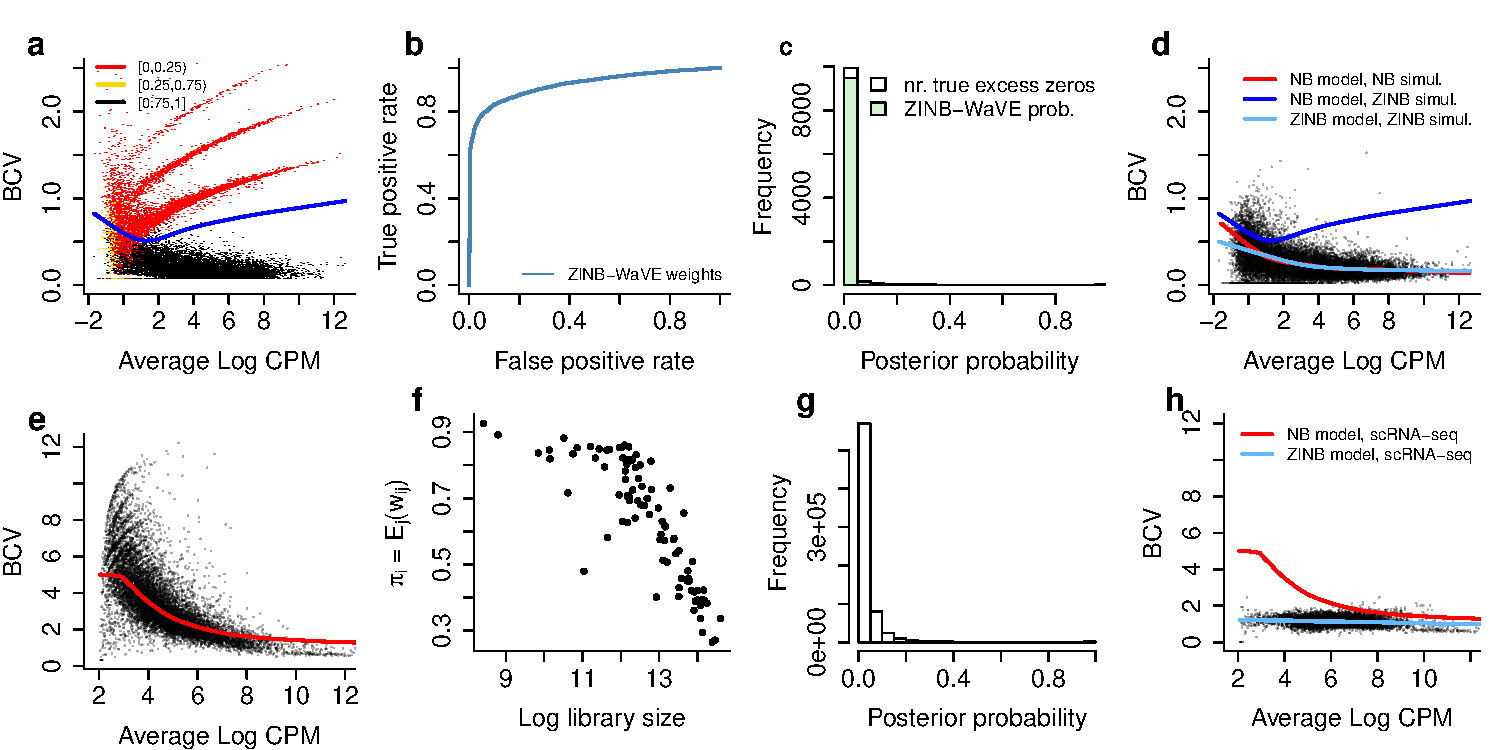
\includegraphics[width=1\textwidth]{../../../figures/introBCV_v2.png}
	%\internallinenumbers
	\caption[introFigure]{Zero-inflation distorts the mean-variance trend in (sc)RNA-seq data but is correctly identified by the ZINB model. The top panels represent simulated RNA-seq data while the bottom panels represent the scRNA-seq dataset from Islam et al. (2011) \cite{Islam2011}. The biological coefficient of variation (BCV) is the square root of the NB dispersion parameter.
	%\textbf{(a)} Simulated RNA-seq dataset for a two-group comparison with five samples in each group. The trend shows high dispersion estimates for lowly expressed genes while a smooth decrease is observed for highly expressed genes.
	\textbf{(a)} Simulated RNA-seq dataset for a two-group comparison with five samples in each group. Randomly replacing 5\% of the expression counts with zeros induces zero-inflation and distorts the mean-variance trend by overestimating the dispersion parameter. The colors represent the average zingeR posterior probability for all zeros from a gene.
	\textbf{(b)} ROC curve for the correct identification of excess zeros, as stratified by the average log CPM. A very good classification precision is obtained for genes with moderate and high expression, while the identification is harder on genes with low expression, since these genes often have higher dispersion estimates.
	\textbf{(c)} Histogram of zingeR posterior probabilities for the excess zeros in the zero-inflated bulk RNA-seq dataset. The white bar at $0$ represents the number of introduced excess zeros. Most excess zeros are identified as such by zingeR, see also Additional File 1: Figure S4.
	%Posterior probabilities on the count component for the introduced zeros in the zero-inflated bulk RNA-seq dataset. Most excess zeros are identified as such by zingeR.
	\textbf{(d)} Effectively downweighting excess zeros using the posterior probabilities recovers the original mean-variance trend and inference on the NB count component will now no longer be biased because of zero-inflation patterns, illustrating zingeR's ability to account for excess zeros.
	\textbf{(e)} BCV plot for the Islam dataset \cite{Islam2011} shows that higher variability is observed in scRNA-seq data as compared to bulk RNA-seq data. As in \textbf{(b)}, zero-inflation induces striped patterns in the BCV plot leading to an overestimation of the dispersion parameter of the count component.
	\textbf{(f)} The sequencing depth of a cell is related to the abundance of zeros, information used by zingeR to identify excess zeros in scRNA-seq datasets when fitting the ZINB model. The pink curve represents the estimated marginal mean on excess zeros for a cell and the difference between the curve and the datapoints represents the estimated expected fraction of zeros that belong to the count component.	
	\textbf{(g)} zingeR posterior probabilities for all zeros in the Islam dataset identify both NB and excess zeros. However, due to the increased noise in scRNA-seq datasets, some zeros are harder to classify as compared to bulk RNA-seq data.
	\textbf{(h)} Using the zingeR posterior probabilities as observation weights results in lower estimates of the dispersion parameter, unlocking powerful differential expression analysis with standard RNA-seq DE methods.
	}
	\label{fig:introBCV}
\end{figure}

\begin{figure}[h!]
	\center
	%\includegraphics[width=1\textwidth]{../../../figures/RNASeq_composite.png}
	%\internallinenumbers
	\caption{ Comparison of methods on simulated RNA-seq data. 
		The left panel (\textbf{a}) shows performance curves on the simulated dataset where $5\%$ of the counts were set to zero. Conventional RNA-seq methods break down due to zero-inflation while most scRNA-seq methods perform reasonably. scde seems to have a good performance in a moderate zero-inflation setting, however it provides very conservative FDR control as suggested by its FDR working points. zingeR\_edgeR outperforms all other methods and in fact performs close to an edgeR analysis based on the truth, where the introduced zeros are effectively downweighted by setting their weights to zero, showing that zingeR\_edgeR correctly identified most excess zeros. A similar result is observed for zingeR\_DESeq2.
	Right panel (\textbf{b}) shows the performance of the evaluated methods on simulated RNA-seq data, suggesting a superior performance of zingeR\_edgeR and providing evidence that the method performs well in non zero-inflation settings. Note, that the working points for zingeR\_DESeq2 are more conservative as compared to DESeq2 due to the use of the t-distribution instead of the Gaussian distribution for the Wald test.
	}
	\label{fig:RNASeqPerf}
\end{figure}



\begin{figure}[h!]
	\center
	%\includegraphics[width=1\textwidth]{../../../figures/scSimulation_composite_cutoff.png}
	%\internallinenumbers
	\caption{Comparison of methods on simulated scRNA-seq data. 
	\textbf{(a)} Performance on scRNA-seq data based on Islam simulation. 
	\textbf{(b)} Performance based on Trapnell simulation. 
	The zingeR workflows clearly outperform other methods in case of severe zero-inflation (a) and are among the best performers in the Trapnell simulation with few excess zeros (b). Note, that the positive counts normalization provides an enormous boost in performance for DESeq2 in the Trapnell simulation. Dedicated methods  scde and metagenomeSeq specifically developed to deal with excess zeros are dominated in both simulations by zingeR workflows and by DESeq2 with positive counts normalization. DESeq2 curves in panel (a) are cut-off due to NA p-values as a result of independent filtering. Full FDP-TPR curves are provided in Additional File 1: Figure S9.}
	\label{fig:scRNASeqPerf}
\end{figure}


\begin{figure}[h!]
	\center
	%\includegraphics[width=1\textwidth]{../../../figures/caseUsoskin_composite.png}
	%\internallinenumbers
	\caption{Case study on neuronal cells. \textbf{(a)} The association of zero abundance with sequencing depth. The three different picking sessions differ in their sequencing depth, causing an attenuated global relationship (blue line). However, accounting for the batch effect in zingeR's zero-excess model, allows for a correct model of sequencing depth with zero abundance. 
	\textbf{(b)} The distribution of posterior probabilities with (white) and without (green) including the batch effect in the zero-excess model. Including the batch effect results in many more zeros being identified as truly zero excess (i.e. the higher bar near a posterior probability of zero) and negative binomial zeros, hence increasing classification certainty.
	\textbf{(c)} False positive rate (FPR) evaluation on $30$ mock comparisons across all cell types. Note, that a different scale is used for metagenomeSeq.}
	\label{fig:usoskin}
\end{figure}


%%%%%%%%%%%%%%%%%%%%%%%%%%%%%%%%%%%
%%                               %%
%% Tables                        %%
%%                               %%
%%%%%%%%%%%%%%%%%%%%%%%%%%%%%%%%%%%

%% Use of \listoftables is discouraged.
%%
%\section*{Tables}

%\begin{table}[h!]
%\caption{Sample table title. This is where the description of the table should go.}
%    \begin{tabular}{cccc}
%        \hline
%           & B1  &B2   & B3\\ \hline
 %       A1 & 0.1 & 0.2 & 0.3\\
  %      A2 & ... & ..  & .\\
  %      A3 & ..  & .   & .\\ \hline
   %   \end{tabular}
%\end{table}

%%%%%%%%%%%%%%%%%%%%%%%%%%%%%%%%%%%
%%                               %%
%% Additional Files              %%
%%                               %%
%%%%%%%%%%%%%%%%%%%%%%%%%%%%%%%%%%%

\section*{Additional Files}
  \subsection*{Additional file 1 --- Supplementary figures and tables}
This file contains all supplementary figures and tables to the manuscript.

\end{backmatter}
\end{document}
